

\begin{figure*}[t] 
        \centering
        \begin{subfigure}[b]{2.0in}
                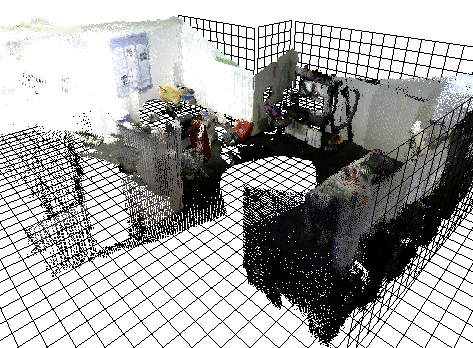
\includegraphics[width=2.0in]{images/ch2/unit21}
                \caption{Apartment}
                \label{fig:RECON_UNIT}
        \end{subfigure}%
        \begin{subfigure}[b]{2.0in}
                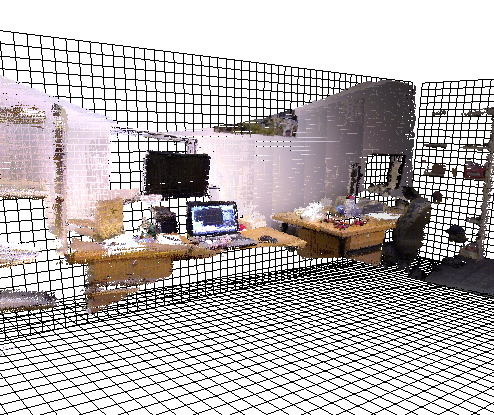
\includegraphics[width=2.0in]{images/ch2/officeA}
                \caption{Office}
                \label{fig:RECON_OFFICE}
        \end{subfigure}%
        \begin{subfigure}[b]{2.0in}
                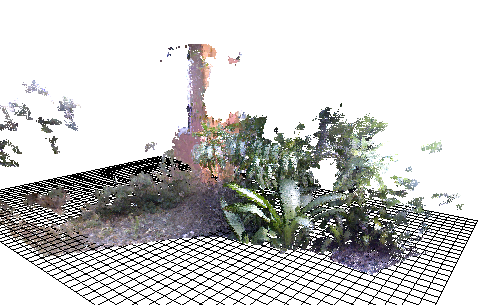
\includegraphics[width=2.0in]{images/ch2/outdoorA}
                \caption{Garden}
                \label{fig:RECON_GARDEN}
        \end{subfigure}
       \caption{Reconstructed Scenes.}
       \label{fig:RECONSTRUCTIONS}
\end{figure*}

Two indoor environments (Apartment and Office) as well as one outdoor environment (Garden) were reconstructed and are shown in figures \ref{fig:RECON_UNIT}, \ref{fig:RECON_OFFICE} and \ref{fig:RECON_GARDEN} respectively. \\

The Apartment reconstruction was recorded by moving through a room and rotating the camera. Some frames contain featureless walls whilst others had contrast shifts due to the camera's automatic contrast feature. Despite these obstacles, accurate reconstruction was achieved. \\

The office reconstruction was also generated by rotating the camera about the y-axis while moving backwards. FVR is a closed form solution yet its accuracy is still comparable to existing feature based SLAM methods. Typical feature based methods work well with indoor environments where local features are readily distinguishable and easy to match. They do not tend to work as well with complex outdoor scenes where feature confusion is likely. To assess performance in such outdoor scenes, a garden scene containing bushes, plants and a ground covering of bark and rocks was used. In the case of a feature matching approach this scene would likely result in feature confusion, making camera tracking difficult. The proposed method was able to produce a good quality reconstruction. Hence, the FVR approach readily overcomes difficulties common to feature matching methods.             
